\documentclass[12pt,a4paper]{article}

\usepackage[utf8]{inputenc}
\usepackage[T1]{fontenc}
\usepackage[swedish]{babel}
\usepackage{amsmath}
\usepackage{amsfonts}
\usepackage{color}
\usepackage{graphicx}
\usepackage{wrapfig}
\usepackage{framed}
\usepackage{pifont}
\usepackage{listings}
\usepackage{subfigure}
%\usepackage{epsfig}
\usepackage[retainorgcmds]{IEEEtrantools}
\usepackage{hyperref}
\usepackage{url}
\hypersetup{colorlinks,
	citecolor=black,
	filecolor=black,
	linkcolor=black,
	urlcolor=black,
	pdftex}
\newcommand{\N}{\ensuremath{\mathbb{N}}}
\newcommand{\Z}{\ensuremath{\mathbb{Z}}}
\newcommand{\Q}{\ensuremath{\mathbb{Q}}}
\newcommand{\R}{\ensuremath{\mathbb{R}}}
\newcommand{\C}{\ensuremath{\mathbb{C}}}
\newcommand{\rd}{\ensuremath{\mathrm{d}}}
\newcommand{\id}{\ensuremath{\,\rd}}
\newcommand{\degree}{\ensuremath{^{\circ}}}
\newcommand{\iu}{\ensuremath{\mathrm{i}}}
\newcommand{\captiona}[1]{\caption{\scriptsize{#1}}}



\begin{document}
	\pagenumbering{roman}

\title{Stelkroppsrörelse i rummet}
	\author{Stefan Buller och Martin Wernstål}
	\date{2011-05-16}
	\maketitle{}
	\thispagestyle{empty}

	\begin{abstract}
	  Stelkroppsrörelse i rummet betraktas. Vi reflekterar över behovet av att inför kroppsfixta 
          koordinater och använder sådana för att ta fram ett speciallfall av Euler ekvationer. Dessa 
          ekvationer används sedan för att betrakta två situation där betrakta kropparna inte har något 
          externt vridande moment. 

          Vi betraktar först speciallfallet då $I_{xx}=I_{yy}$ och härleder en 
          relation mellan precession och spinn längsmed huvudsymmetriaxeln. Denna relation används sedan 
          för att ta fram jordens precessionshastighet i vår modell, som visar sig vara $1,0034$ varv per dygn. 

          Vi betraktar sedan en faktisk kropps rotation efter det att den givits en begynnelsehastighet kring en av sina axlar.
          För den axeln med det mellanliggande vridmomentet finner vi att rotationsvektorn ändrar sig signifikant under ett 
          kastförlopp. Detta speglas i modellen av att problemet blir instabilt då kroppens initialla rotationshastighet 
          är förhållandevis större i denna riktning.
	\end{abstract}

\newpage{}

	\tableofcontents{}
	\thispagestyle{empty}

\newpage{}

	\setcounter{page}{1}
	\pagestyle{plain}
	\pagenumbering{arabic}
	
	
\section{Problem 1}
	\subsection{Delproblem a}
	I ett kroppsfixt koordinatsystem, gäller som namnet antyder, att punkter på kroppen
	har en fixt position i förhållande till koordinatsystemet. Då deras positionsvektorer
	inte ändras kan man räkna ut integralerna ingående i tröghetsmatrisen utan något tidsberoende.

	\subsection{Delproblem b}
	$M = \dot{L}$, och då vi valt att uttrycka $L$ i ett kroppsfixt koordinatsystem $xyz$ får vi
	bidrag i $\dot{L}$ dels från $\mathbf{L}$:s förändring i de kroppsfixa koordinataxlarna
	$\hat{x},\hat{y},\hat{z}$ och dels från koordinataxlarnas förändring i det omgivande
	koordinatsystemet.
	
	Låt $\omega$ vara $xyz$:s rotationsvektor, och därmed även kroppens rotationsvektor.
	
	Detta ger oss vridmomentekvationen:
	
	\begin{equation*}
		M = \dot{L} = \dot{L}_{xyz} + \omega \times L
	\end{equation*}
	
	
	Komponentvist, då vi har ett koordinatsystem som sammanfaller med kroppens huvudtröghetsaxlar:
	
	\begin{equation}
		\begin{cases}
			M_x = I_{xx}\dot{\omega}_x + (I_{zz} - I_{yy})\omega_y\omega_z \\
			M_y = I_{yy}\dot{\omega}_y + (I_{xx} - I_{zz})\omega_z\omega_x \\
			M_z = I_{zz}\dot{\omega}_z + (I_{yy} - I_{xx})\omega_x\omega_y
		\end{cases}
		\label{vridmomentsekvationerna_komponentvis}
	\end{equation}
	
\section{Problem 2}
	\subsection{Delproblem a}
	Symmetriaxel-fixt koordinatsystem $\hat{x},\hat{y},\hat{z}$ med $I_{xx} = I_{yy} = I_0$ och $I_{zz} \neq I_0$:
	
	\begin{equation*}
		I = \begin{bmatrix}
			I_0 & 0 & 0 \\
			0 & I_0 & 0 \\
			0 & 0 & I_{zz}
		\end{bmatrix}
	\end{equation*}
	
	Låt $\boldsymbol{\nu}$ vara kroppens rotation i det symmetri-axel-fixa koordinatsystemet,
	$\boldsymbol{\omega}$ vara kroppens rotation relativt det omgivande inertialsystemet samt $\mathbf{\Omega}$ vara
	$\hat{x}\hat{y}\hat{z}$-systemets rotation.
	
	Eftersom $\hat{x}\hat{y}\hat{z}$ är symmetriaxel-fixt så måste $\nu_x = \nu_y = 0$ för att
	systemet skall fortsätta att vara symmetriaxel-fixt.
	
	\begin{IEEEeqnarray*}{rCl}
		\boldsymbol{\omega} & = & \mathbf{\Omega} + \boldsymbol{\nu} \\
		\mathbf{M} & = & \dot{\mathbf{L}}_{xyz} + \mathbf{\Omega} \times \mathbf{L} \\
		& = & I \boldsymbol{\dot{\omega}} + \boldsymbol{\Omega} \times I \boldsymbol{\omega} \\
		& = & \begin{cases}
			I_x \dot{\omega}_x + \Omega_y I_z \omega_z - \Omega_z I_y \omega_y\\
			I_y \dot{\omega}_y + \Omega_z I_x \omega_x - \Omega_x I_z \omega_z\\
			I_z \dot{\omega}_z + \Omega_x I_y \omega_y - \Omega_y I_x \omega_x
		\end{cases}
	\end{IEEEeqnarray*}
	
	Vi betraktar fallet då $\mathbf{M} = \mathbf{0}$ och $\Omega$ konstant relativt $\hat{x}\hat{y}\hat{z}$-systemet:
	
	\begin{equation*}
		\begin{cases}
			0 = I_0 \dot{\omega}_x + \Omega_y I_z \omega_z - \Omega_z I_0 \omega_y\\
			0 = I_0 \dot{\omega}_y + \Omega_z I_0 \omega_x - \Omega_x I_0 \omega_z\\
			0 = I_z \dot{\omega}_z + \Omega_x I_0 \omega_y - \Omega_y I_x \omega_x
		\end{cases}
		\hspace{12pt}
		\Rightarrow
		\hspace{12pt}
		\begin{cases}
			0 = \Omega_y I_z (\Omega_z + \nu_z) - \Omega_z I_0 \Omega_y \\
			0 = \Omega_z I_0 \Omega_x - \Omega_x I_0 (\Omega_z + \nu_z) \\
			0 = I_z \dot{\nu}_z + \Omega_x \Omega_y (I_0 - I_0)
		\end{cases}
	\end{equation*}
	
	Vilket ger:
	
	\begin{equation}
		\frac{\Omega_z}{\nu_z} = \frac{I_z}{I_0 - I_z}
		\hspace{24pt}
		\mathrm{och}
		\hspace{24pt}
		\dot{\nu}_z = 0
\label{IoejIz}
	\end{equation}
	\subsection{Delproblem b}
	Då vi har kroppsfixt system utan yttre vridande moment bör precessionsvektorn
	gå igenom kroppens masscentrum.  Då vi har ett värde för precessionsvektorn i 
        rotationsvektorns riktning enligt \eqref{IoejIz}, samt dess riktning i förhållande 
        till rotationvektorns riktning, så får vi precessionsvektorns uttryckt i 
        symmetriaxelfixta systemet $\hat{x}\hat{y}\hat{z}$:
	
	\begin{equation*}
		\Omega_z = \frac{\nu_z I_z}{I_o-I_z}
		\hspace{12pt}
		\Omega_x = \frac{b \nu_z I_z}{R(I_o-I_z)}
		\hspace{12pt}
		\Omega = \frac{\nu_z I_z R \cos(b/R)}{I_o-I_z}
	\end{equation*}
	Med beteckningar enligt figur \ref{jorden}.

	Enligt förutsättningarna är det ett avstånd på 10 meter mellan rotation och
	precessionsvektor vid jordytan, $b=10 \,\mathrm{m}$. Radien vid polerna är $R_p= 6356,7523 \,\mathrm{km}$ \footnotemark[1],
	radien vid ekvatorn: $R_e=6378,1370 \,\mathrm{km}$ \footnotemark[1]. För att få jordens tröghetsmoment integrerar över en homogen ellipsoid.
\footnotetext[1]{Källa: \url{http://en.wikipedia.org/wiki/Earth_radius\#Fixed_radii}}
	Fås att $I_o = \frac{m}{5}(R_p^2+R_e^2), I_z = \frac{2m}{5}R_e^2$ vilket ger relativa
	skillnaden: $\frac{I_o-I_z}{I_z} = -0,0033472$, samt att $\Omega \approx -299\nu$. Om
	$\omega=\Omega+\nu = \frac{2\pi}{24 \,\mathrm{h}}$ ger detta att
	$\nu \approx \frac{-\frac{2\pi}{298}}{24 \,\mathrm{h}}$, alltså spinner jorden ett cirka varv på 300
	dagar i motsatt riktning till precessionen. Precessionshastigheten blir då $\frac{-598\pi}{298 \cdot 86400 \,\mathrm{s}} = 7,2966 \cdot 10^{-5}$, eller $1,0034$ varv per dygn.

	\begin{figure}
		\begin{center}
			\input{jordb.pstex_t}
			\caption{Förhållandet mellan precessionaxeln $R_p$ och rotationsaxeln $z$}
                        \label{jorden}
		\end{center}
	\end{figure}

	\subsection{Delproblem c}
		För en godtycklig precessionsvektor $\boldsymbol{\Omega}= \Omega_x \hat{x} + \Omega_y \hat{y} + \Omega_z \hat{z}$
		och för ett symmetriaxel-fixt 
		koordinatsystem har vi endast spinn kring huvudsymmetriaxeln, $\boldsymbol{\nu}=\nu \hat{z}$.
		Detta ger oss kroppens absoluta rotation: 
		$\boldsymbol{\omega}=\Omega_x \hat{x} + \Omega_y \hat{y} + (\Omega_z + \nu )\hat{z}$, kroppens rörelsemängd moment: 
		$\mathbf{L}=I_o \Omega_x \hat{x} + I_o \Omega_y \hat{y} + I_z (\nu + \Omega_z) \hat{z}$.
		Låt $\hat{z}$ och $\mathbf{n} := \Omega_x \hat{x} + \Omega_y \hat{y}$ 
		spänna ett plan. Våra vektorer kan alla uttryckas i dessa vektorer, alltså ligger de alltid i samma plan i de symmetriaxelfixa koordinatsystemet. 
		
		
		För att dra slutsatser om vilka som är fixta i ett inertialsystem så tar vi tidsderivatan av
		vektorerna. Vi har enligt förutsättningen att $\mathbf{M} = \dot{\mathbf{L}} = \mathbf{0}$ ,
		dvs $\mathbf{L}$ är fixt. Övriga vektorer är det inte, $\dot{\hat{z}}=\boldsymbol{\Omega} \times \hat{z}$,
		vilket inte är noll då precessionsaxeln avviker från $\hat{z}$. $\dot{\boldsymbol{\omega}} = \dot{\boldsymbol{\Omega}}+\dot{\boldsymbol{\nu}} =
		0 + \boldsymbol{\Omega} \times \nu \hat{z}$, är inte noll av samma skäl.
		Man kan även resonera kring att de 3 alltid ligger i ett plan som är fixt i 
		ett symmetriaxelfixt system precesserande system, alltså inte utanför systemet.
		
		Sett innefrån ett system som roterar med $\boldsymbol{\omega}$ så blir $\hat{z}$ fixt, ty det enda som skilljer vårt kroppsfixta system från 
		vårt symmetriaxelfixta är att vi nu har en axel i $\hat{z}$ riktning som roterar, men i övrigt sammanfaller den med $\hat{z}$ som alltså alltid pekar upp ur samma punkt.
		Då $\mathbf{L}$ och $\boldsymbol{\omega}$ alltid låg i ett och samma plan spänt av $\hat{z}$ och $\hat{y}$ med komponenter i $\hat{y}$-led, så kan de inte vara fixta i vårt kroppsfixta system som bara ibland har en axel i $\hat{y}$ led.
		

	
\section{Problem 3}
	
	
	\subsection{Experiment}
		
		Vår studerade kropp är ett homogent rätblock med dimensionerna
		$a = 0,25 \mathrm{m}$, $b = 0,08 \mathrm{m}$, $c = 0,01 \mathrm{m}$.
		
		Vi inför ett kroppsfixt koordinatsystem med origo i masscentrum med axlarna
		$\hat{x}$, $\hat{y}$ och $\hat{z}$ som går genom den största, näst
		största respektive minsta ytan.
		
		Enligt vårt experiment roterar vår kropp stabilt kring $\hat{x}$ och $\hat{z}$, men
		instabilt kring $\hat{y}$.
		
		\begin{figure}
			\begin{center}
				\includegraphics[width=0.5\textwidth]{Photo1.eps}
				\caption{Det använda homogena rätblocket}
			\end{center}
		\end{figure}
		
	\subsection{Beräkningar}
		
		Våra uppmätta värden för kroppen ger tröghetsmoment genom masscentrum:
		
		\begin{equation*}
			\begin{cases}
				I_x = \frac{1}{12} m (a^2 + b^2) \\
				I_y = \frac{1}{12} m (a^2 + c^2) \\
				I_z = \frac{1}{12} m (b^2 + c^2) 
			\end{cases}
			\hspace{12pt}
			\Rightarrow
			\hspace{12pt}
			\begin{cases}
				I_x = \frac{1}{12} m (\frac{689}{10000}) \\
				I_y = \frac{1}{12} m (\frac{626}{10000}) \\
				I_z = \frac{1}{12} m (\frac{65}{10000})
			\end{cases}
		\end{equation*}
		
		Yttre moment $\mathbf{M}=\mathbf{0}$ ger:
		
		\begin{equation*}
			\begin{cases}
				I_x \dot{\omega}_x = \omega_y \omega_z (I_y - I_z) \\
				I_y \dot{\omega}_y = \omega_z \omega_x (I_z - I_x) \\
				I_z \dot{\omega}_z = \omega_x \omega_y (I_x - I_y)
			\end{cases}
			\hspace{12pt}
			\Rightarrow
			\hspace{12pt}
			\begin{cases}
				\dot{\omega}_x = \omega_y \omega_z \gamma_x \\
				\dot{\omega}_y = \omega_z \omega_x \gamma_y \\
				\dot{\omega}_z = \omega_x \omega_y \gamma_z
			\end{cases}
		\end{equation*}
		
		\begin{IEEEeqnarray*}{lClCl}
			\gamma_x = \frac{I_y - I_z}{I_x} &\hspace{24pt}&
			\gamma_y = \frac{I_z - I_x}{I_y} &\hspace{24pt}&
			\gamma_z = \frac{I_x - I_y}{I_z} \\
			\gamma_x \approx 0,81778 & &
			\gamma_y \approx -0,99681 & &
			\gamma_z \approx 0,96923
		\end{IEEEeqnarray*}
		
		Trivialt fall är om vi har en ren vinkelhastighet i något led, då fås ingen
		vinkelaccelleration i vår modell.
		
		Dominerande vinkelhastigheter i $x$- eller $z$- led kommer att få $\dot{\omega}_y$
		att växla tecken samt befinna sig nära noll. Säg att:
		
		$(\omega_x(t_0) > \omega_y(t_0) > 0) \land (\omega_x(t_0) > \omega_z(t_0) > 0)$, vilket leder till att
		
		\begin{center}
		\begin{tabular}{l|lll}
			Tid & $\omega_x$ & $\omega_y$ & $\omega_z$  \\
			\hline
			$t_0$ & $+\nearrow$ & $+\searrow$ & $+\nearrow$ \\
			$t_1$ & $+\searrow$ & $-\searrow$ & $+\searrow$ \\
			$t_2$ & $+\nearrow$ & $-\nearrow$ & $-\searrow$ \\
			$t_3$ & $+\searrow$ & $+\nearrow$ & $-\nearrow$ \\
			\hline
			$t_4$ & $+\nearrow$ & $+\searrow$ & $+\nearrow$ \\
			$\vdots$ & & $\vdots$ &
		\end{tabular}
	\end{center}
		
		$t_1$ är tillfället då $\omega_y$ korsar noll, $t_2$ är tillfället då $\omega_z$ korsar
		noll ($\omega_x$ korsar aldrig noll ty $\omega_x > \omega_z$) och $t_3$ då $\omega_y$
		ytterligare en gång korsar noll-linjen. Detta resulterar i tidpunkten $t_4$ vilket är
		tillfället då vi är tillbaka till ursprungstillståndet. 
		
		Systemet är alltså stabilt då $|\omega_x| \gg |\omega_y| \land |\omega_x| > |\omega_z|$.
		Analogt gäller för $|\omega_z| > |\omega_x|$.
		
		Om vi däremot inte har större
		vinkelhastigheter i $x$- och $y$-led så kommer $\dot{\omega_y}$ inte bli negativt
		nog och svängingsrörelsen blir oregelbunden. Problemet blir instabilt: små
		begynnelsevärden i $x$ och $y$-led ger stora utslag. Detta överänsstämmer väl med
		det vi observerade.
		
		Ändring i hastighetsriktning kommer från att att kroppen spinner runt och därför
		ändrar orientering; en observatör utanför koordinatsystemet skulle inte märka
		några plötsliga ändringar i hastighetens riktning.
		
		\begin{equation}
			\dot{\boldsymbol{\omega}}^{\prime} = \begin{bmatrix}
				0 & \omega_z \gamma_x & \omega_y \gamma_x \\
				\omega_z \gamma_y & 0 & \omega_x \gamma_y \\
				\omega_y \gamma_z & \omega_x \gamma_z & 0
			\end{bmatrix}
			\label{jacobian}
		\end{equation}
		
		Om vi nu vill beräkna stabiliteten av vårt system beräknas då egenvärdena av
		Jacobianmatrisen \eqref{jacobian} och stabiliteten är $\mathrm{max} (\lambda_i),\,i \in \{1,2,3\}$.
		
		\begin{figure}
			\begin{center}
				\subfigure[$\hat{x}$-rotation]{\label{fig:x}\includegraphics[width=0.3\textwidth]{simulated/1_std.eps}}
				\hspace{12pt}
				\subfigure[$\hat{y}$-rotation]{\label{fig:y}\includegraphics[width=0.3\textwidth]{simulated/2_std.eps}}
				\hspace{12pt}
				\subfigure[$\hat{z}$-rotation]{\label{fig:z}\includegraphics[width=0.3\textwidth]{simulated/3_std.eps}}
				\\
				\subfigure[Störd $\hat{x}$-rotation]{\label{fig:x-per}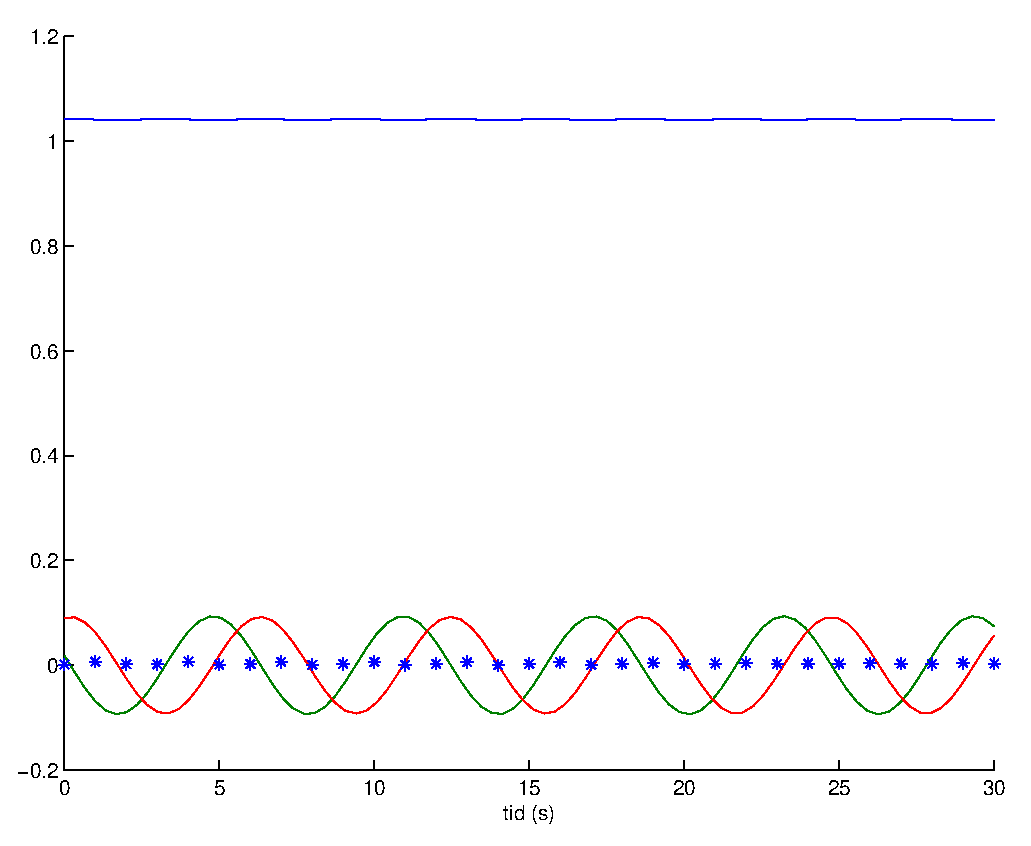
\includegraphics[width=0.3\textwidth]{simulated/1_per.eps}}
				\hspace{12pt}
				\subfigure[Störd $\hat{y}$-rotation]{\label{fig:y-per}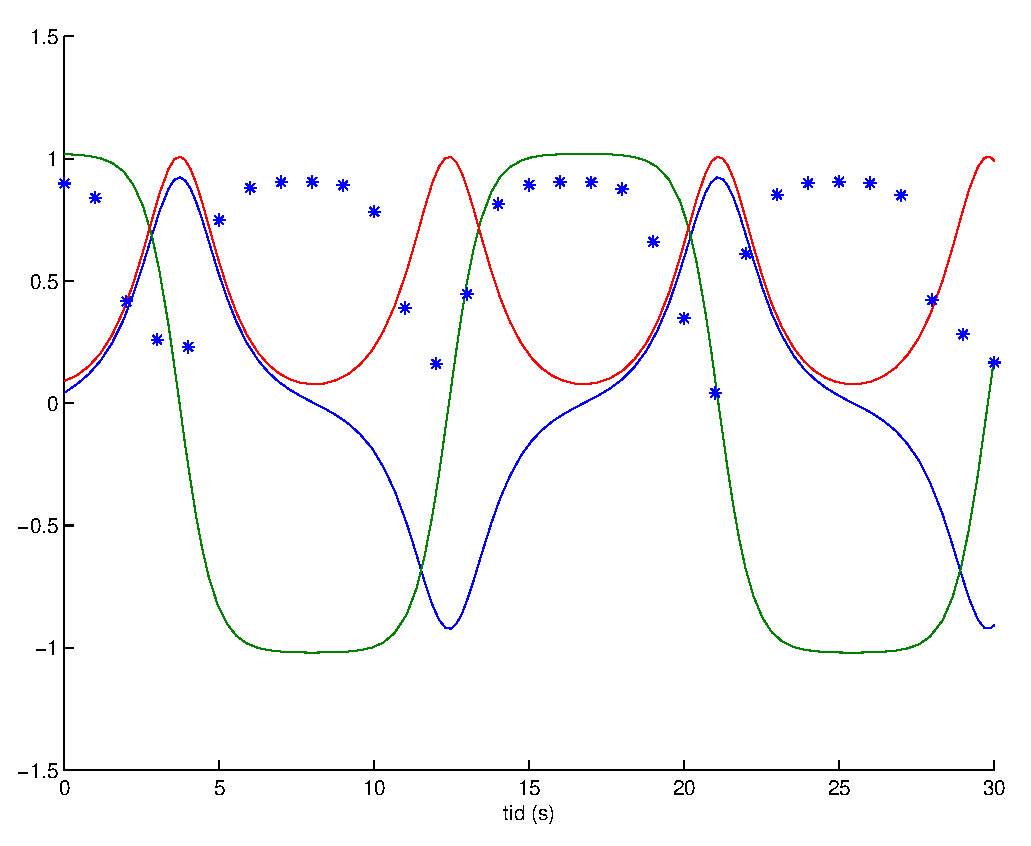
\includegraphics[width=0.3\textwidth]{simulated/2_per.eps}}
				\hspace{12pt}
				\subfigure[Störd $\hat{z}$-rotation]{\label{fig:z-per}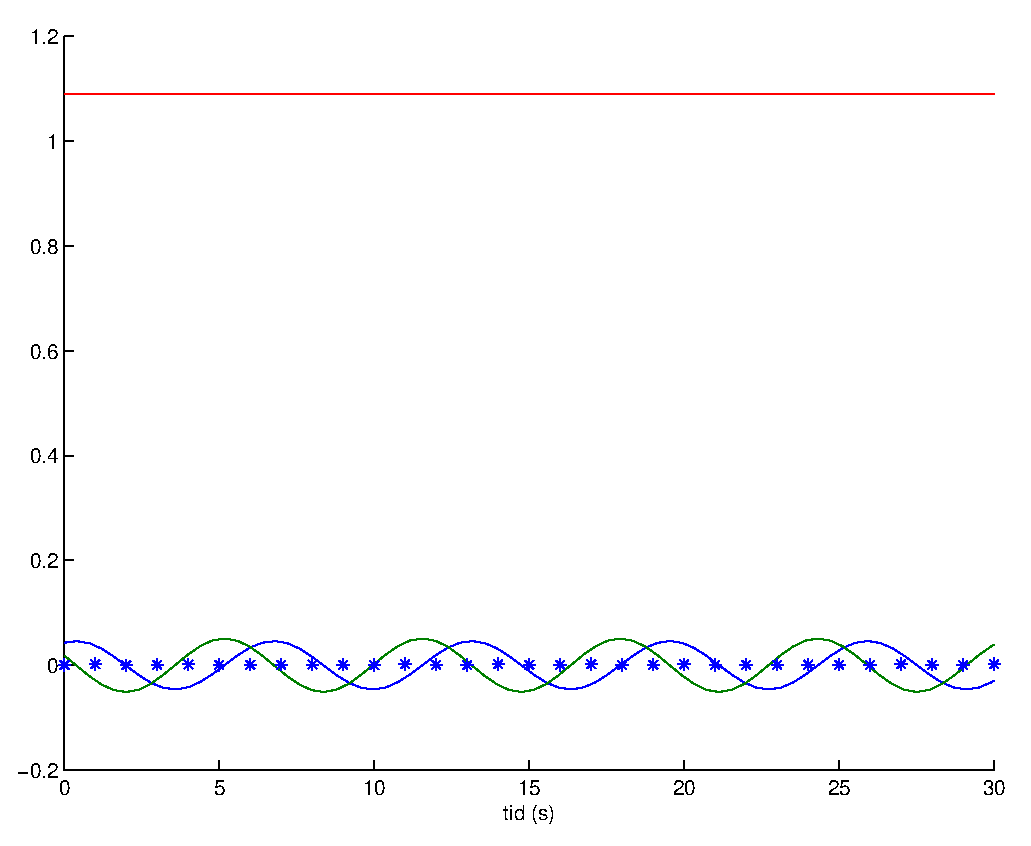
\includegraphics[width=0.3\textwidth]{simulated/3_per.eps}}
			\end{center}
			\caption{Rotationer runt de tre olika symmetriaxlarna, blå $=\hat{x}$-rotation, grön $=\hat{y}$-rotation,
			röd $=\hat{z}$-rotation. Prickarna representerar stabilitet i diskreta punkter, där 0 och under är stabilt.}
		\end{figure}
		
		Även extremt små störningar av $\hat{y}$-rotation (i storleksordningen $10^{-10}$) påverkar rotationen markant,
		förutsatt att den får fortsätta i minst en minut.
		
		% Resonera kring graferna
		
\pagebreak

\begin{appendix}
	\section{MATLAB-simuleringskod}
	
		\lstset{
		  literate={ö}{{\"o}}1
		           {å}{{\aa}}1
		           {ä}{{\"a}}1
		}
		
		\lstset{language = MATLAB,
		        commentstyle = \textit,
		        showspaces = false,
		        showstringspaces = false,
		        showtabs = false,
		        tabsize = 2,
		        basicstyle = \scriptsize,
		        breaklines,
		        breakatwhitespace,
		        postbreak = \ding{229},
		        extendedchars = true
		}
		
		\begin{framed}
			\lstinputlisting[]{simulate.m}
		\end{framed}
		
\end{appendix}
\end{document}
